\chapter{Methodology}
\label{ch:Methodology}
This chapter builds on the findings from the \textit{Literature Review} in \autoref{ch:LiteratureReview}, outlining the key ideas and concepts needed to achieve the research objectives. The specifics of implementing these methodologies will be discussed in detail in the next chapter. \par

\section{Explorative Approach}
\label{sec:ExplorativeApproach}
\begin{figure}[ht]
    \centering
    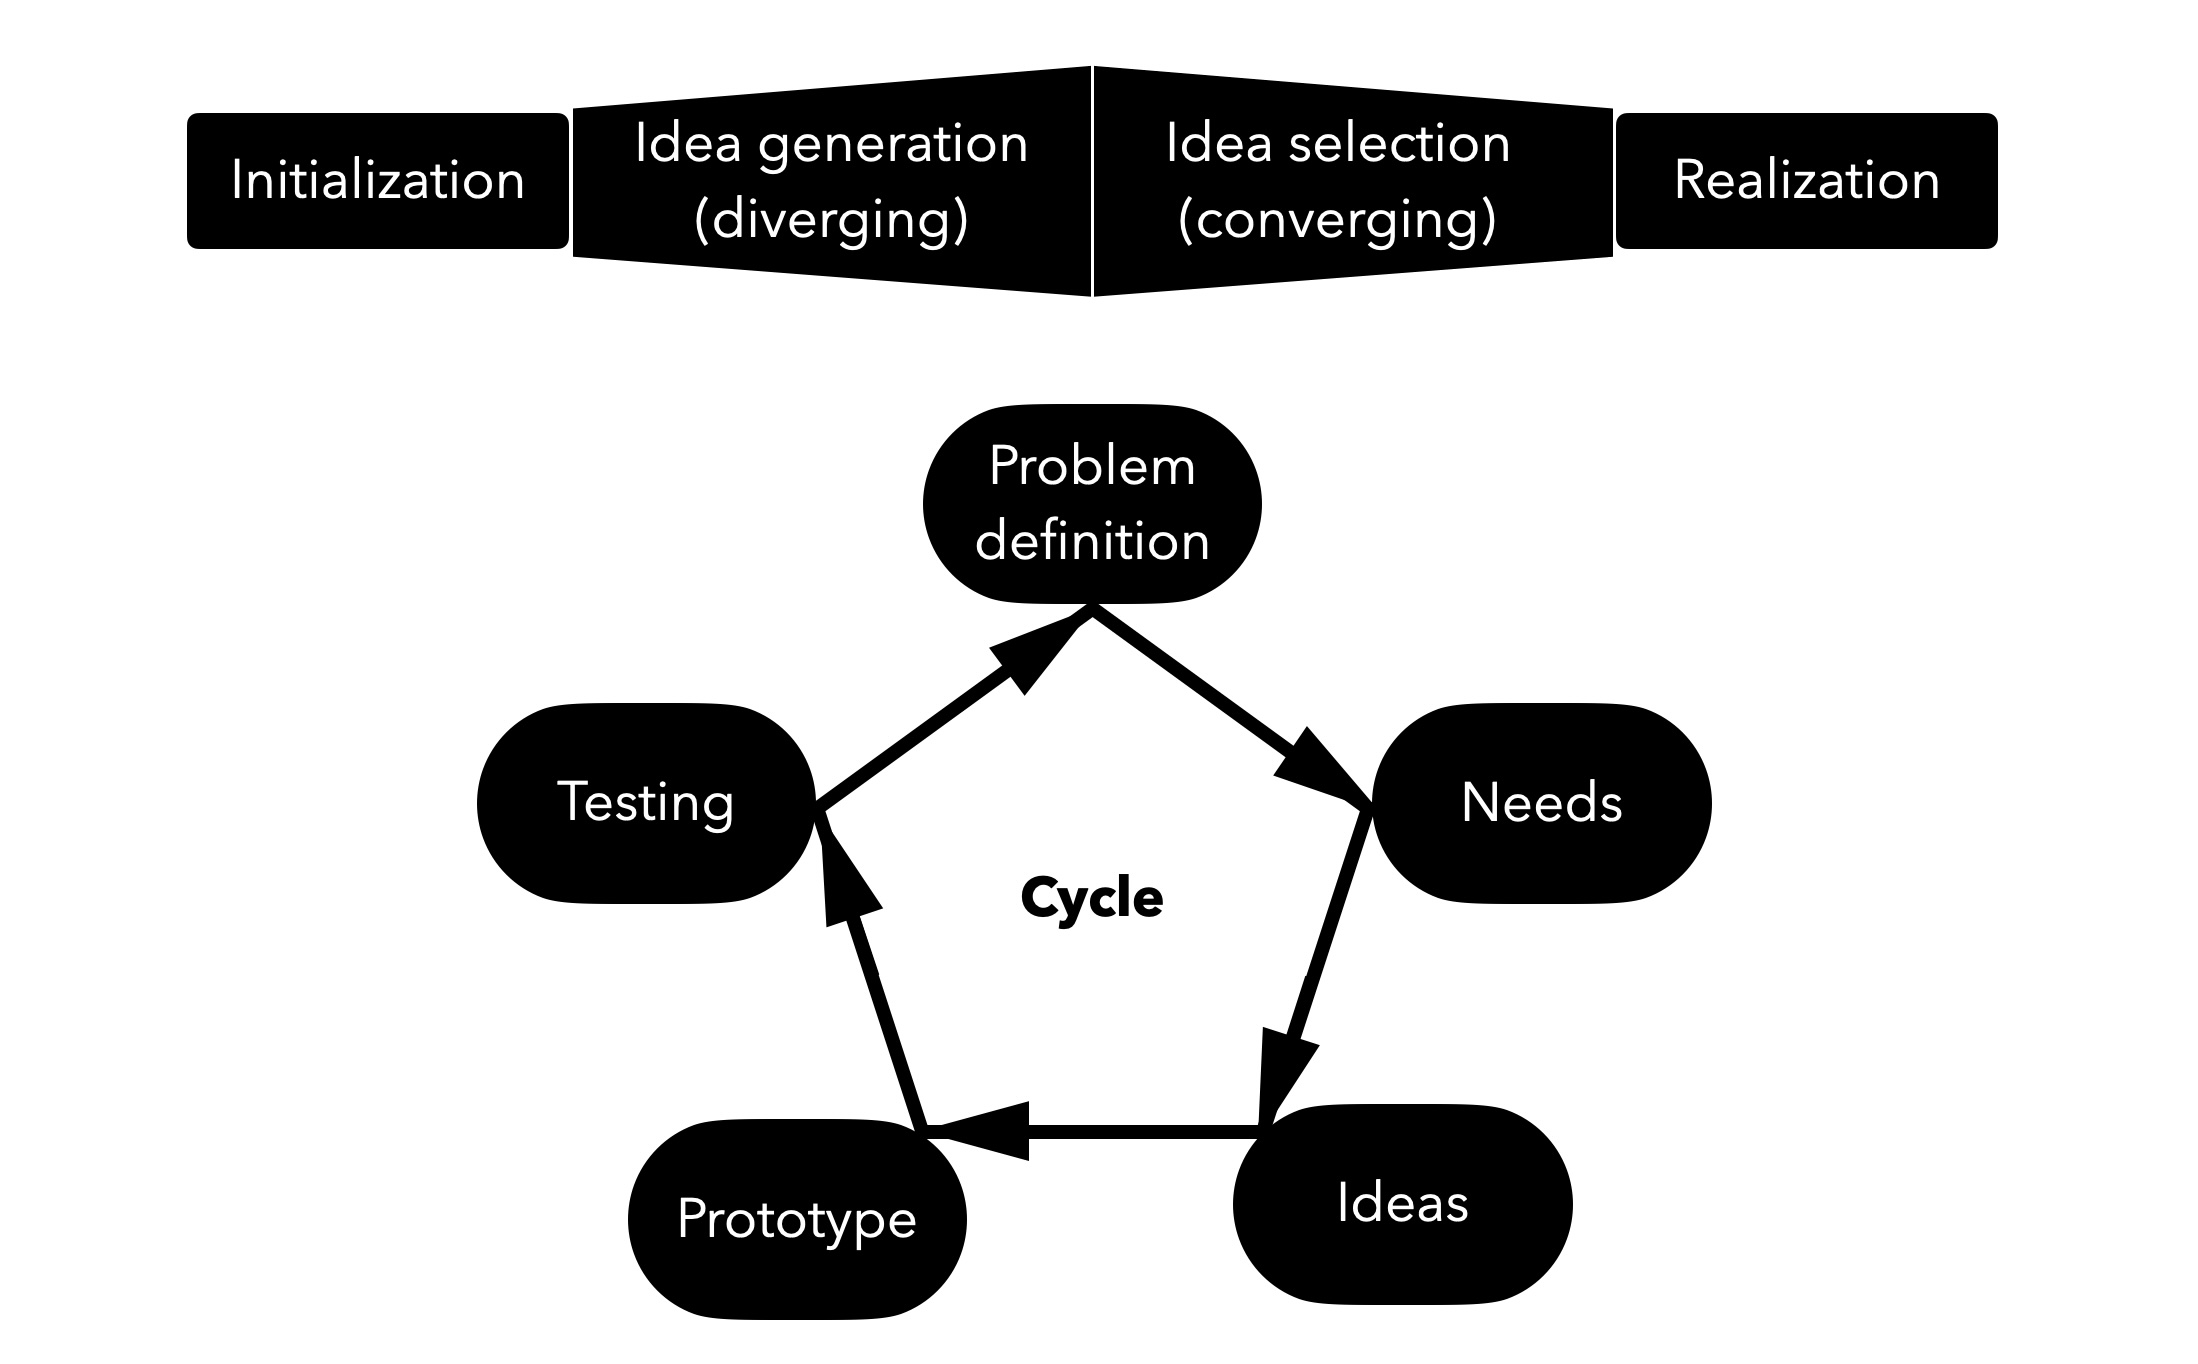
\includegraphics[keepaspectratio,width=13cm]{img/DecisionCycle.jpg}
    \caption{Visualization of the explorative approach, including the stages of initialization, idea generation, idea selection, and implementation. The lower part of the figure shows the decision cycles adapted from \autocite{DesignThinking}.}
    \label{fig:decision_cycle}
\end{figure}
\noindent
IQA, particularly in the context of teledermatology, presents many opportunities for innovation because of the diverse types of image distortions and the different methods available to address them. To navigate this complexity, this research uses an exploratory approach. This approach is flexible and allows for changes as new information becomes available. This is different from more traditional methods like the “waterfall model,” which follows a strict, step-by-step process.\par
\vspace{\baselineskip}
\noindent
At the beginning, the problem was defined in broad terms to allow flexibility and adaptability. As the research progressed,  the approach involved creatively solving problems and refining methods through multiple cycles of learning and improvement. The project was structured into two main phases: \par
\begin{itemize}
    \item \textbf{Idea Generation Phase}:  During this phase, the scope of the research questions was broadened to continuously generate new ideas. This expansion was driven by insights gathered from the ongoing literature review.
    \item \textbf{Idea Refinement Phase}: This phase focused on combining and refining these ideas into clear findings and conclusions, aiming to develop a comprehensive understanding of the initial problem.
\end{itemize}
\noindent
This exploratory model is shown in \autoref{fig:decision_cycle}, which shows the stages of starting the project, generating ideas, selecting the best ideas, and implementing them. It also shows the decision cycles that guide the project \autocite{DesignThinking}. These cycles help in adjusting the research direction based on new findings and insights, making sure that the methodology stays responsive to new data and trends. \par 

\section{Project Control}
\label{sec:ProjectMonitoring}
Even with an exploratory approach, it is important to have a rough timeline to guide the research tasks. A workflow was set up before starting, and a detailed Gantt chart is attached to this thesis to show the timeline. \par
\vspace{\baselineskip}
\noindent
For the first half of the research, three key milestones were set, each playing a critical role for its success: \par
\vspace{\baselineskip}
\noindent
\textbf{Understanding Teledermatology}: Gaining a thorough understanding of teledermatology is necessary. This makes sure that all subsequent actions are relevant and well-informed. \par
\vspace{\baselineskip}
\noindent
\textbf{State of the Art in IQA}: Identifying the latest developments in IQA is very important. This helps makes sure that the methods used are up-to-date and effective. \par
\vspace{\baselineskip}
\noindent
\textbf{Availability of Teledermatology Images}: Securing access to appropriate datasets is necessary for conducting meaningful IQA. Having the right images is important for testing and validating the research methods. \par
\vspace{\baselineskip}
\noindent
These milestones are important because each phase of the project depends on the successful completion of the previous one. Missing any of these milestones could significantly impact the project and might require a fundamental reassessment of the objectives outlined in \autoref{sec:Objectives}. \par

\clearpage
\section{Research Steps}
\label{sec:ResearchSteps}
As mentioned, this research was exploratory, so it was not possible to follow a strict, step-by-step process. However, a systematic approach was taken for the key steps to stay organized and ensure each step was done in the right order. \par

\subsection{Literature Review}
\label{sub:LR}
The first step was to gain a comprehensive understanding of the research field. Teledermatology and dermatology can be complex areas, so it was essential to build a strong foundation of knowledge. This was done by extensively researching and reading relevant literature to develop a solid understanding of these fields. Additionally, the same approach was taken for understanding IQA. The goal was to learn about the main topics related to the research objectives.\par
\vspace{\baselineskip}
\noindent
To find relevant literature, several databases were selected, including PubMed\footnote{https://pubmed.ncbi.nlm.nih.gov}, Google Scholar\footnote{https://scholar.google.com}, IEEE Xplore\footnote{https://ieeexplore.ieee.org/Xplore/home.jsp}, Connected Papers\footnote{https://www.connectedpapers.com}, and Papers with Code\footnote{https://paperswithcode.com}. Search filters were applied to narrow down the results, such as limiting the search to articles published after 2020. Special attention was given to state-of-the-art methods, especially those that had published their code and model details. This helped in accessing practical resources and the latest research.\par
\vspace{\baselineskip}
\noindent
This systematic approach provided a thorough literature review, focusing on the most relevant and up-to-date studies. \par

\subsection{Data Collection and Preparation} 
\label{sub:DataCollection}
In the general image domain, IQA commonly uses labels like Mean Opinion Score (MOS) or Differential Mean Opinion Score (DMOS) to train models. However, in the medical field, labeling images with these scores is resource-intensive, so dermatology datasets typically do not have these score labels. \par
\vspace{\baselineskip}
\noindent
To address this gap, a distortion pipeline was created to synthetically distort images based on the seven dermatology quality criteria defined in \autoref{sub:QualityCriteriaTeledermatology}. Each type of distortion has five levels of severity, indicating how poor the image quality is. These distortions are carefully selected to simulate real-world imperfections commonly encountered in teledermatology. Each image is then labeled with seven values corresponding to the severity and type of distortion applied, creating a dataset that includes both the distorted images and precise annotations regarding their quality. \par
\vspace{\baselineskip}
\noindent
To start with, good quality images were needed. Two datasets were chosen for this purpose: the SCIN \autocite{SCIN} dataset for its relevance and uniqueness, and the Fitzpatrick17k \autocite{F17K} dataset to complement the SCIN dataset. Filtered good quality images from these datasets were passed through the distortion pipeline, creating different versions of distortions for each image. This approach means that the original number of images can be expanded significantly through synthetic distortion, allowing for a more robust training and evaluation process. \par 
\clearpage
\noindent
In total, 475 good quality images were filtered from the Fitzpatrick17k \autocite{F17K} dataset and another 475 good quality images from the SCIN \autocite{SCIN} dataset for training and evaluation. Additionally, 200 test images were selected from the SCIN dataset and 70 independent good quality images from SCIN dataset for testing. The 70 good quality images were also fed through the distortion pipeline to introduce synthetic distortions, providing a consistent basis to test the model against the same types of distortions. Furthermore, the 200 test images were labeled, scoring each one on the seven dermatology quality criteria to allow the model’s performance to be also compared to human evaluation. \par
\begin{table}[ht]
    \centering
    \begin{tabular}{|l|l|}
        \hline
        \textbf{Dataset} & \textbf{Description} \\
        \hline
        SCIN\textsubscript{good} & 475 good quality images filtered from the SCIN dataset. \\
        F17K\textsubscript{good} & 475 good quality images filtered from the Fitzpatrick17k dataset. \\
        SCIN\textsubscript{distorted} & Synthetic distortions applied to SCIN\textsubscript{good}. \\
        F17K\textsubscript{distorted} & Synthetic distortions applied to F17K\textsubscript{good}. \\
        COMB\textsubscript{distorted} & Combined synthetic distortions. \\
        \hline
        SCIN\textsubscript{authentic} & 200 test images labeled with human evaluation scores. \\
        SCIN\textsubscript{synthetic} & 70 good quality test images, synthetically distorted. \\
        \hline
    \end{tabular}
    \caption{Summary of the datasets used in the research. Note that the Fitzpatrick17k dataset is referred to as F17K for simplicity.}
    \label{table:dataset_summary}
\end{table}

\subsection{Feature Extraction}
\label{sub:FeatureExtraction}
Feature extraction is the next important step where the state-of-the-art approach from ARNIQA \autocite{ARNIQA} is used to identify key features from the synthetically distorted images. ARNIQA is chosen because it has been trained on many different types of image distortions. This training allows ARNIQA to recognize and understand different distortion patterns effectively. By using ARNIQA, this knowledge can be applied to teledermatology images, improving the ability to assess image quality. \par
\vspace{\baselineskip}
\noindent
The features extracted by ARNIQA capture the patterns of distortions that affect image quality. These features, along with the generated labels from the synthetic distortion pipeline, are then used to train different models, including Extreme Gradient Boosting (XGBoost) regressor, XGBoost classifier, and Multi-Layer Perceptron (MLP) regressor and MLP classifier. By training and comparing these models, the most effective approach for assessing image quality in teledermatology can be identified. \par

\subsection{Training and Validation}
\label{sub:TrainVal}
The training of the models is based on the prepared training images. Because labels and distorted images are generated, there is no restriction on the original number of images. The images can be passed through the distortion pipeline multiple times, creating different versions of distortions from the original images. This allows for a larger and more diverse training set.\par 
\vspace{\baselineskip}
\noindent
The models are then trained using these distorted images to develop their ability to assess image quality. Validation is done alongside training by setting aside a portion of the data as a validation set. This validation set helps to evaluate and monitor the performance of the models, ensuring they are learning correctly and adjusting as needed. \par

\subsection{Evaluation Metrics}
\label{sub:EvaluationMetrics}
The evaluation of the models is done using defined metrics such as Mean Absolute Error (MAE), R-squared (R\textsuperscript{2}), Spearman’s Rank Order Correlation Coefficient (SRCC), and Cohen’s Kappa. These metrics help understand the strengths and weaknesses of the models and guide further improvements or adjustments. \par
% I want to mention in the subsub section the individual metrics and how the help in evaluating the model.
\subsubsection{Understanding the Metrics and Their Importance}
\label{subsub:UnderstandingMetrics}
\textbf{MAE} measures the average difference between the predicted image quality scores and the actual scores. It helps in understanding how accurate the models’ predictions are on average. A lower MAE indicates better model performance, meaning the predictions are closer to the actual values. \par
\vspace{\baselineskip}
\noindent
\textbf{R\textsuperscript{2}} indicates how well the predicted scores match the actual data. It tells us how much of the variance in the actual scores is explained by the models’ predictions. A higher R\textsuperscript{2} means better model performance, showing that the model’s predictions fit the actual data well. Using MAE and R\textsuperscript{2} together provides a clear picture of the model’s accuracy and how well it fits the actual data. \par
\vspace{\baselineskip}
\noindent
\textbf{SRCC} measures the strength and direction of the association between two ranked variables. In simpler terms, it evaluates how well the predicted rankings of image quality match the actual rankings. For example, if the model predicts the severity of distortions in the same order as the actual severity, it will have a high SRCC. SRCC is calculated as: \par
\begin{equation}
    SRCC = 1 - \frac{6 \sum_{i=1}^n (d_i^2)}{n(n^2 - 1)}
\end{equation}
\noindent
where, \newline
$n: \text{Number of images} \\ d_i: \text{Difference in ranks between predicted and actual scores for image } i$ \par
\vspace{\baselineskip}
\noindent
An SRCC of 1 means perfect rank correlation, and -1 means perfect negative correlation. This metric is crucial because, in many cases, getting the rank order correct is more important than predicting the exact value. If images are ranked correctly in terms of severity, even if the predicted values are not exact, the model can still be useful in prioritizing cases for further review. \par
\vspace{\baselineskip}
\noindent
\textbf{Cohen’s Kappa} measures how well the models’ predictions agree with the actual labels. Unlike SRCC, which focuses on ranking, Cohen’s Kappa evaluates the exact agreement between predictions and actual labels. Unlike simple accuracy, which only looks at the proportion of correct predictions, Cohen’s Kappa accounts for the possibility that some agreement might occur by chance. It is calculated as: \par
\begin{equation}
    Kappa = \frac{p_o - p_e}{1 - p_e}
\end{equation}
\noindent
where, \newline
$p_o: \text{Observed agreement} \\ p_e: \text{Expected agreement}$ \par
\vspace{\baselineskip}
\noindent
Cohen’s Kappa ranges from -1 to 1, with 1 indicating perfect agreement and 0 indicating agreement by chance. \par

\subsection{Testing and Evaluation}
\label{sub:TestExperiment}
After completing the training, the models are evaluated using independent test images. There are two test sets used in this evaluation. The first test set consists of images that have been synthetically distorted to simulate common types of distortions. The purpose of this test set is to assess the performance and reliability of the models when faced with consistent types of distortions. By using this controlled environment, it’s possible to see how well the models handle different distortion levels. \par 
\vspace{\baselineskip}
\noindent
The second test set includes real-world images with authentic distortions. The performance of the models on this test set is compared to human evaluations. This comparison helps to understand how well the models’ assessments align with human judgment, providing a more realistic measure of their effectiveness. The results from these test sets are then compared using radar charts to visualize the models’ strengths and weaknesses across different quality criteria. \par

\subsection{Model Comparison}
\label{sub:basecomp}
To compare the performance of the image quality assessment model for teledermatology, a baseline comparison was done against two methods: Structural Similarity Index Measure (SSIM) and ARNIQA \autocite{ARNIQA}. This helps to show how effective the proposed approach is and where it can be improved. \par 
\vspace{\baselineskip}
\noindent
SSIM is a widely-used method that compares the similarity between two images by measuring changes in structure, brightness, and contrast. It can only be used when both the original image and its distorted version are available. ARNIQA, on the other hand, is a pre-trained No-Reference Image Quality Assessment (NR-IQA) method that gives quality scores without needing the original image. \par 
\vspace{\baselineskip}
\noindent
The comparison involves plotting the single quality scores from the proposed model, SSIM, and ARNIQA, as well as calculating the Spearman’s Rank Correlation Coefficient (SRCC) to see how well the predicted scores match the true quality scores. This comparison also helps to understand where the proposed model does better or needs improvement compared to traditional and state-of-the-art methods. \par
\vspace{\baselineskip}
\noindent
In addition to these comparisons, an out-of-distribution test was done. Images that are different from the training data, taken from the KADID10K \autocite{KADID10k} dataset, were used for this test. These images include nature scenes, vehicles, animals, and everyday objects. The model’s predictions on these unrelated images were checked to see if the model produces reasonable scores or shows large differences, which could mean the model is too specialized to the teledermatology domain. \par

\subsection{Discussion and Further Development}
\label{sub:DiscussionDevelopment}
In conclusion, the results of the project are analyzed and discussed. This discussion includes an evaluation of the achieved goals, an analysis of the challenges and limitations of the project, and a look at possible further developments. \par
